%% An Introduction to LaTeX Thesis Template of Wuhan University
%%
%% Created by WHUTUG

\documentclass[type=bachelor]{whu-thesis}
\usepackage[noend]{algpseudocode}
\usepackage{algorithmicx,algorithm}
\whusetup
  {
    info               =
      {
        title          = {基于咳嗽音音频分析的哮喘检测},
        title*         = {},
        student-number = {2017301500098},
        school         = {计算机学院},
        author         = {张建},
        author*        = {},
        subject        = {计算机科学与技术},
        major          = {计算机科学与技术},
        advisor        = {张健 , 教授},
        direction      = {研究方向},
        % date           = {2021/3},
        keywords       = {哮喘检测,咳嗽音频,音频分析,迁移学习,VGG网络 , 机器学习,支持向量机},
        keywords*      = {Asthma Detection, Cough audio, Audio Analysis, Transfer Learning, VGG Network, Machine Learning, Support Vector Machine},
      },
    style              =
      {
        graphics-path  = {{figures/}{data/}},
        list-of-figures,
        list-of-tables,
      },
    element            =
      {
        innovation     = {pages/innovation},
        abstract       = {pages/abstract},
        abstract*      = {pages/enabstract},
        bibliography   = {ref/refs , ref/thu},
        achievements   = {pages/achievements},
        thanks         = {pages/thanks},
        appendix       = {pages/appendix}
      }
  }

\begin{document}
%%----------- 主体部分 ----------- %%
% Chapter 1

\chapter{绪论}

\section{引言}
哮喘是现代社会常见一种呼吸道疾病,患者常有喘息、咳嗽、呼吸短促等症状。因为其具有高发病率,持续时间长和反复发作等特性\cite{louis2000relationship},已经成为了严重的社会公共卫生问题。同时在所有的患者中只有25\%$ \sim $50\%患者被医生知晓,众多的患者在早期未被诊断前会出现肺功能逐步下降等病理现象,这对于患者的恢复与治疗产生了更大的挑战。\cite{van2003detection}

长期以来,医务人员已经认识到人体声音可以作为健康的指标。例如,使用听诊器听取来自心脏或肺部的声音\cite{pramono2017automatic}。但是这些通常需要熟练的临床医生进行聆听和诊断,并近期迅速被各种成像技术所替代,诸如 MRI、超声检查等。而对于这些新兴技术而言,分析和诊断疾病更加容易,但是并不适用于大规模的潜在患者的筛选,不具有经济性和便捷性。用自动音频特征建模技术将会给个人的日常生活工作的疾病监测提供巨大的潜力。

同时智能手机和可穿戴设备已经被广泛的使用于人体信号监测,例如:呼吸波形\cite{xu2019breathlistener}、脉搏\cite{BloodGlucoseMonitoringSystem}、肌肉振动\cite{barry1992muscle}等身体信号。例如:在breathListener\cite{xu2019breathlistener}中,手机麦克风和扬声器生成ESD信号对人体胸腔的运动变化进行监测,生成了精度高的人体呼吸波形。但是以上研究仅仅局限于提高数据收集精度,而并没有用于实际的医学诊断和治疗中,作为一种有潜力且最方便的信号监测工具,智能手机可以作为一般用户自我诊疗的辅助系统,加强普遍场合下健康诊断的可靠性。

为了解决以上痛点,本论文实现了一种基于音频特征建模技术的哮喘检测方法。对比与传统的哮喘检测方法,音频特征建模技术具有易于测量、诊断时间短、特异性强等优势:
\begin{enumerate}
  \item \textbf{易于测量}:一般来说,咳嗽音的频率低于20kHz,而一般的智能手机麦克风的采样频率在40kHz左右。因此,本研究可以直接应用智能手机的麦克风进行咳嗽音的采样,并将咳嗽音重采样至22kHz,极大的拓展了哮喘检测的使用场景和应用范围。
  \item \textbf{诊断时间短}:对于已经生成的分类模型,将测试好的音频输入模型进行处理、分类,可以在2分钟内返回诊断结果。
  \item \textbf{特异性强}:前期研究实验表明,即使咳嗽不是自发的,也就是哮喘患者被要求咳嗽时,它仍然含有哮喘的特定特征\cite{bales2020can}。这意味着受试者可以通过模拟咳嗽的方法来对哮喘进行筛选检测,并且具有一定的稳定性与特异性。
\end{enumerate}

\section{本论文的主要工作}
本论文实现了一种基于音频特征建模技术的哮喘检测方法,其主要工作和贡献概述如下:
\begin{enumerate}
  \item \textbf{采样应用实现}:基于Android Studio平台,实现了一款名为asthma sound的安卓应用,采样3次咳嗽的录音存储到手机本地内存。
  \item \textbf{音频数据增强}:由于采样数据有限,系统在检测采样音频为咳嗽音后,将采样音频重新定位到22kHz,采用原始信号放大,添加白噪音,更改音调和速度共三种方法增强音频\cite{schluter2015exploring}。在合理的范围内将每种方法分别应用2次,将数据量扩增6倍,用于原始模型的训练,从而大大提高模型的鲁棒性。
  \item \textbf{音频特征提取}:基于librosa\cite{mcfee2015librosa}音频处理库,利用重采样的音频在帧和段层次使用MFCC提取各种音频特征,同时利用VGG网络自动提取其他维度的音频特征,共提取了733维的特征向量,最后采用主成分分析(PCA)法进行降维,用于音频分类。
  \item \textbf{特征分类网络实现}:对于所有提取到的特征向量,系统使用支持向量机(SVM)进行二分类,并且使用K折交叉验证,减少数据的过拟合,分类出哮喘与健康人群。
  \item \textbf{分类模型评估}:对于本模型实现的二分类模型,统计所有的特征数据的分类结果,并统计为混淆矩阵进行分析。混淆矩阵共有四个分量:TP(实际为正预测为正),FP(实际为负但预测为正),TN(实际为负预测为负),FN(实际为正但预测为负)。具体如图\ref{fig:zhibiao}所示。
  
\end{enumerate}
\begin{figure}[h]
  \centering
  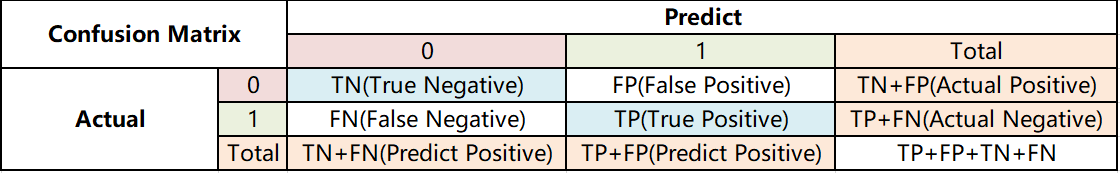
\includegraphics[width=\textwidth]{figures/指标.png}
  \caption{模型评估指标}
  \label{fig:zhibiao}
\end{figure}
\section{文本组织架构}
本文基于对近期研究热点音频特征建模技术,将其与目前健康检测领域的痛点相结合,并聚焦于目前一种常见的呼吸道疾病——哮喘,提出了一种基于音频特征建模的哮喘检测系统。该论文的总体组织结构如下:

第一章为绪论。本章简单介绍了当前健康检测领域的发展现状,并分析了当前健康检测领域的痛点和音频特征建模技术的优势。最后介绍了本论文的主要工作点。

第二章为理论基础。本章首先介绍音频特征建模工作的基础,然后介绍音频数据增强方法,并分析音频增强方法对实验结果的影响、最后介绍深度卷积网络VGG的基本原理,并简单分析利用VGG提取音频特征的原因。

第三章为系统设计。本章首先介绍本论文系统的整体架构,然后分模块介绍最重要的四个部分:咳嗽音频获取与筛选、咳嗽音频的数据增强、特征提取网络的架构以及特征分类网络的架构。

第四章为实验设计及其结果。本章介绍如何利用k-折交叉验证设计实验验证设计模型的有效性;并将结果进行分析说明

第五章为总结与展望。本章对本文的研究工作进行总结,分析了本文提出模型的优缺点。并在该课题下对本研究未来的方向提出了新的展望。

% Chapter 2
\chapter{理论基础}
\section{音频特征建模基础}
在深度学习领域,音频特征建模常用于语音识别等领域。目前市面常见的虚拟助手:Siri、小爱同学和图灵机器人等,都是构建于音频特征建模的基础上。在音频分类、语言合成和语言认识方面,音频特征建模已经很成熟了。
在深度学习领域,音频特征建模常用于语音识别等领域。目前市面常见的虚拟助手:Siri、小爱同学和图灵机器人等,都是构建于音频特征建模的基础上。在音频分类、语言合成和语言认识方面,音频特征建模已经很成熟了。基于音频处理库——Librosa ,本部分主要介绍音频特征建模的理论基础:数字信号处理、滤波器和 Mel 图\cite{mcfee2015librosa}

\begin{figure}[h]
  \centering
  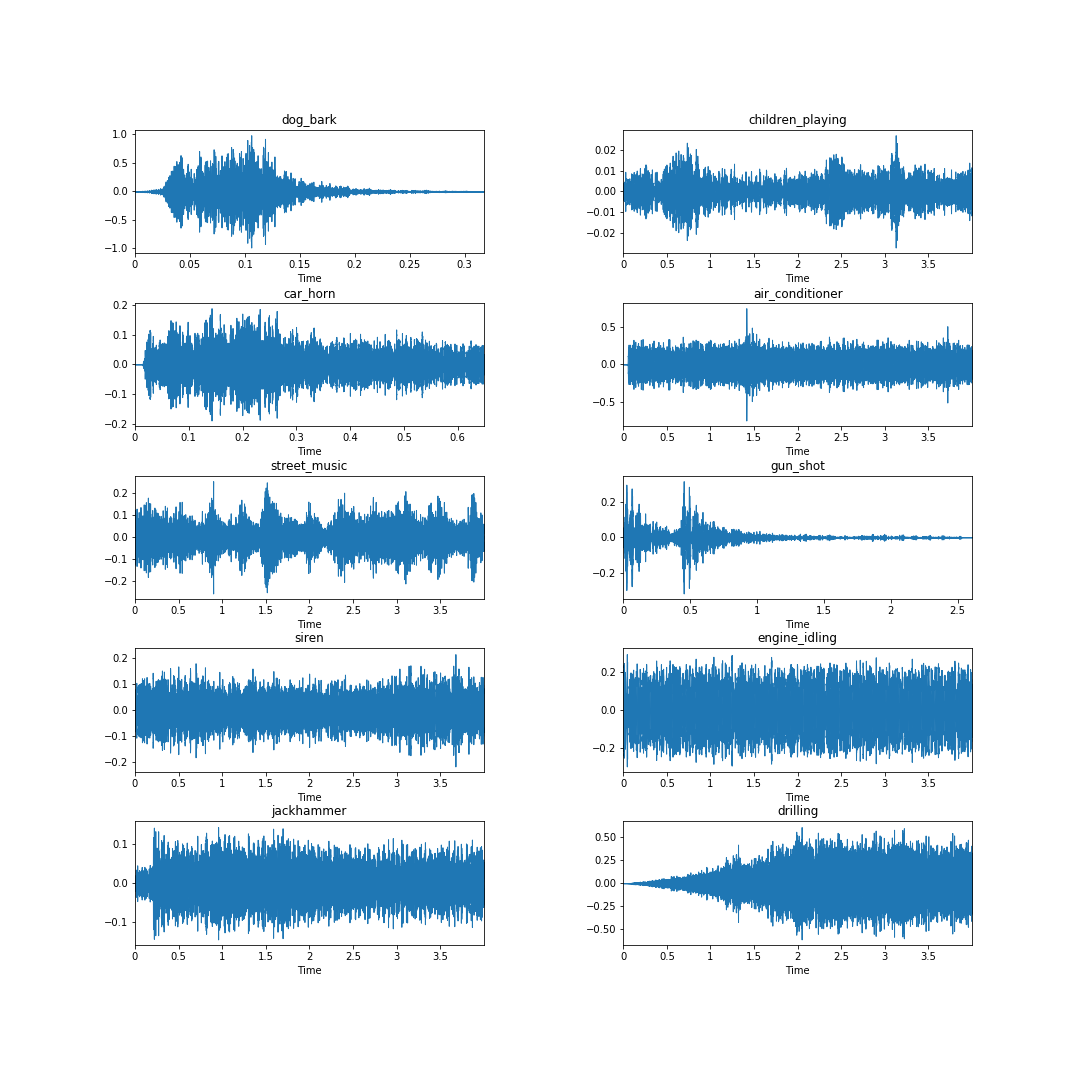
\includegraphics[width=0.7\textwidth]{figures/基础音频.png}
  \caption{常见音频的波形图}
  \label{fig:boxingtu}
\end{figure}

\subsection{从原始音频说起}
常见的音频主要是利用手机麦克风,在40kHz左右的采样频率下进行收集的。因此呈现在 wav 文件中常常是以一维的格式利用扬声器进行输出。从人眼观察的角度来看,音频样本具有着一定的周期性和特征性,但是更精细的信息都是人眼无法去分别出来的,图图\ref{fig:boxingtu}中有个十种音频信号的波形图,通过肉眼观察,引擎声、报警器声和空调声看上去非常的相似。以下音频信号的概念是常见用于描述波形图的特征的术语。
\begin{enumerate}
  \item \textbf{采样和采样频率}:在音频信号处理中,采样是将连续信号按一定规律记录信号使之成为一组离散值而采样频率就是这个采样的规律即一定时间内采样的个数。一般常见手机麦克风的采样频率在40kHz左右。 
  \item \textbf{幅值}: 音频波形的幅度是固定时间内波形变化的量度。幅度的另一个常用定义是变量的极差的大小。一般为了比较相对度的大小,系统会在音频处理种把幅度分量进行归一化处理。
      \begin{figure}[h]
      \centering
      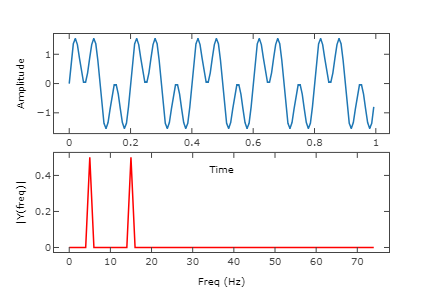
\includegraphics[width=0.7\textwidth]{figures/傅里叶变换图片.png}
      \caption{傅里叶变换示例}
      \label{fig:fuliye}
    \end{figure}
  \item \textbf{傅里叶变换}:原始声音波形往往只能看到其随时间变化规律,而看不出来其频率的变化规律。傅里叶变换就是为了展示其频率变化的一种方法。
        \begin{equation}
         F(w) = \digamma[f(t)] = \int_{-\infty}^{ +\infty} f(t)e^{-iwt} dx
         \label{eq:2.1}
        \end{equation}
        
    傅里叶变换的理论基础是将所有信号看作任意多个三角函数的叠加。因此傅里叶变换是一种将信号投影到三角函数(基)的方法。公式\eqref{eq:2.1}中w表示频率,t表示时间,\eqref{eq:2.1}中将信号表示为三角基函数的叠加。
    对于一个非周期信号,可以将非周期信号看成一个周期信号的一部分。即:傅里叶变换当周期足够大,就会退化为一般情况下的信号函数。因此傅里叶级数退化为:
    \begin{equation}
        f(t) = \sum_{k=-\infty}^{\infty} C_k e^{2\pi(K/T)t}
    \end{equation}
    
    其中\(C_k\)为傅里叶级数,其表示为:
    \begin{equation}
        C_k  = \frac{1}{T}\int_{0}^{T} e^{-2\pi i(\frac{k}{T})t}f(t) d t
        = \frac{1}{T}\int_{-\frac{2}{T}}^{-\frac{2}{T}} e^{-2\pi i(\frac{k}{T})t}f(t) d t
    \end{equation}
    图\ref{fig:fuliye}是利用matlab生成的周期音频信号。上图是一个周期音频信号,下图是该信号的变换结果。

    \item \textbf{周期图}:周期图是基于傅里叶变换的方法。它对音频信号直接做傅里叶变换并且进行平方,如公式\ref{eq:2.4}:
        \begin{equation}
            S_{pre}(w) = \frac{1}{N}|c_k|^2
            \label{eq:2.4}
        \end{equation}
    其中\(C_k\)是傅里叶级数。周期图代表了一个音频在频率方向上密度的估计,即图\ref{fig:zhouqitu}表示的是图\ref{fig:fuliye}中音频信号的周期图。
    \begin{figure}[h]
      \centering
      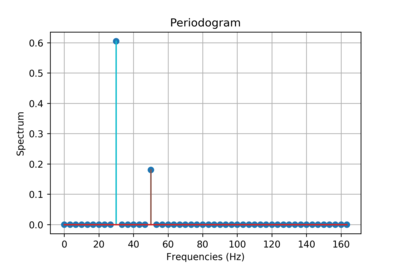
\includegraphics[width=0.7\textwidth]{figures/周期图图片.png}
      \caption{周期图示例}
      \label{fig:zhouqitu}
    \end{figure}
    \item \textbf{梅尔倒频谱系数}:由于人耳对等距离音高感官并不是非线性的。在1980年Davis和Mermelstei\cite{zheng2001comparison}提出一种定义:将1000Hz 且比人类听觉阈值高40分贝高的音频信号定义为1000mels。当频率大于500Hz时,每当人耳感觉到相同的音高变化量时,所需的频率变化就会随着频率的增加而变得越来越大。 
            \begin{equation}
            m = 2595\log_{10}{(1+\frac{f}{700})}
            \label{eq:2.4}
        \end{equation}
    图\ref{fig:mel1}是频率到Mel的映射关系图。从图中可以看到,在频率较低时,Mel随频率变化较快;当频率较高时,斜率变小,变化缓慢\cite{zheng2001comparison}。
     \begin{figure}[h]
      \centering
      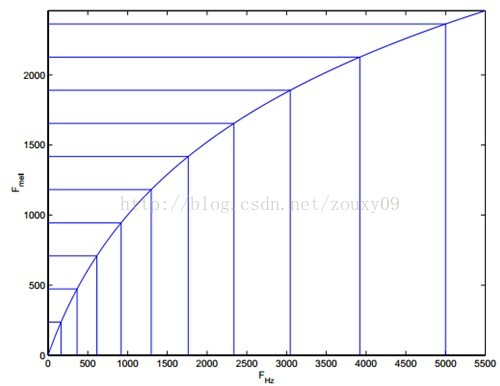
\includegraphics[width=0.7\textwidth]{figures/mel1.jpg}
      \caption{频率:Mel 关系示意图}
      \label{fig:mel1}
    \end{figure}
\end{enumerate}

\subsection{音频特征提取之Mel图}
音频特征提取的一个重要方面就是:梅尔频谱系数(MFCC)的计算,而利用MFCC可以求出Mel图。Mel图与其他一般的音频特征提取方法相比共有以下优势:
\begin{enumerate}
    \item 对于音频的特征进行了去除相关度并进行压缩,更加方便后续的处理。
    \item 适合数据量更小的样本集。
    \item MFCC具有低维度,在频谱上显示的更加平整。
\end{enumerate}
MFCC实现的基本流程图如下图\ref{fig:MFCC},按照预加重、分频加窗、离散傅里叶变换和三角空间滤波、离散余弦变换共五步。
     \begin{figure}[h]
      \centering
      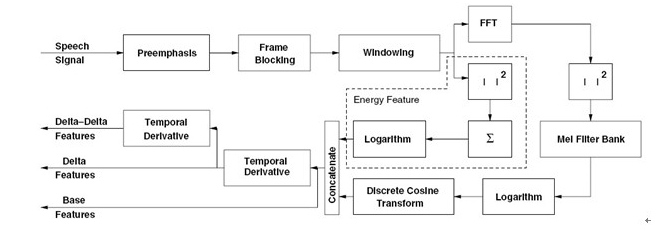
\includegraphics[width=\textwidth]{figures/MFCC.jpg}
      \caption{MFCC实现流程图}
      \label{fig:MFCC}
    \end{figure}
\begin{enumerate}
    \item \textbf{预加重}:由于音频信号在发声过程中会受到嘴唇等身体部位的干扰,需要通过一种高通滤波器来强化高频部分。这样处理后的音频信号会显示的更加平坦,滤波公式为公式\ref{eq:hz}
    \begin{equation}
        H(Z) = 1 - \mu z^{-1}
        \label{eq:hz}
    \end{equation}
    \item \textbf{分帧加窗}:由于手机的采样频率是44.1KHz,即每秒采样44.1K个点,而一般采样的音频频率为22kHz。又因为一个标准帧的长度为25ms。所以每帧有\(22000*0.025 = 550\)个采样点。分帧操作就是对每帧按照10ms的跨度进行拆分。假设声音信号为\(s(n)\),完成分帧操作后为\(s_i(n)\);
    \item \textbf{离散傅里叶变换}:对\(s_i(n)\)做离散傅里叶变换得到\(S_i(k)\),对应的功率密度为\(P_i(k)\);
    \begin{equation}
        S_i(k) = \sum_{n=1}^N s_i(n)h(n)e^{-j2{\pi}kn/N}
    \end{equation}
    \begin{equation}
        P_i(k) = \frac{1}{N}|S_i(k)|^2
    \end{equation}
    对分帧后的数据还需要按帧乘以汉明窗。这种方法可以显著提高帧左右段的连续性,实现公式如下
    \begin{equation}
        S_i(k) = S_i(k)\times W_i(k)
    \end{equation}
    \begin{equation}
        W_i(k,a) = (1-a)-a\times \cos{\frac{2\pi n}{N-1}}
    \end{equation}
    这里的a一般取为0.5
    \begin{figure}[h]
      \centering
      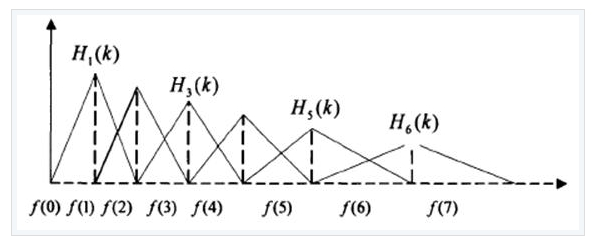
\includegraphics[width=\textwidth]{figures/三角滤波器.jpg}
      \caption{三角滤波器组的设置}
      \label{fig:sanjiao}
    \end{figure}
    \item \textbf{三角空间滤波}:通常使用26个左右的三角滤波器,对\(P_i(k)\)进行滤波,根据公式\ref{eq:2.4},可以求出MEL最大为\(f_{max}[mel] = 2146.1mel\),由于三角空间滤波的设置往往是等间隔的处理,所以其频率的间隔为公式\ref{eq:mel}
    \begin{equation}
        \delta = \frac{f_{max}}{\kappa+1}=93.3 mel
        \label{eq:mel}
    \end{equation}
    同时可对相邻三角空间滤波的上限频率进行设置
    \begin{equation}
        c(l) = h(l-1)=o(l+1)
    \end{equation}
    具体如图\ref{fig:sanjiao}所示

    \item \textbf{离散余弦轩变换}:在求离散余弦变换前需要计算每个滤波器组输出的对数能量
    \begin{equation}
        s(m) = ln(\sum_{k=0}^{N-1}|X_a(k)|^2H_m(k))
    \end{equation}
    其中\(0\le m \le M\),之后利用DCT求得MFCC系数:
    \begin{equation}
        C(k) = \sum_{m=0}^{n-1}s(m)\cos{\frac{\pi k(m-0.5)}{M}}
    \end{equation}
\end{enumerate}
由此对图\ref{fig:fuliye}进行mel图谱的构建,其结果如图\ref{fig:Mel}所示
     \begin{figure}[h]
      \centering
      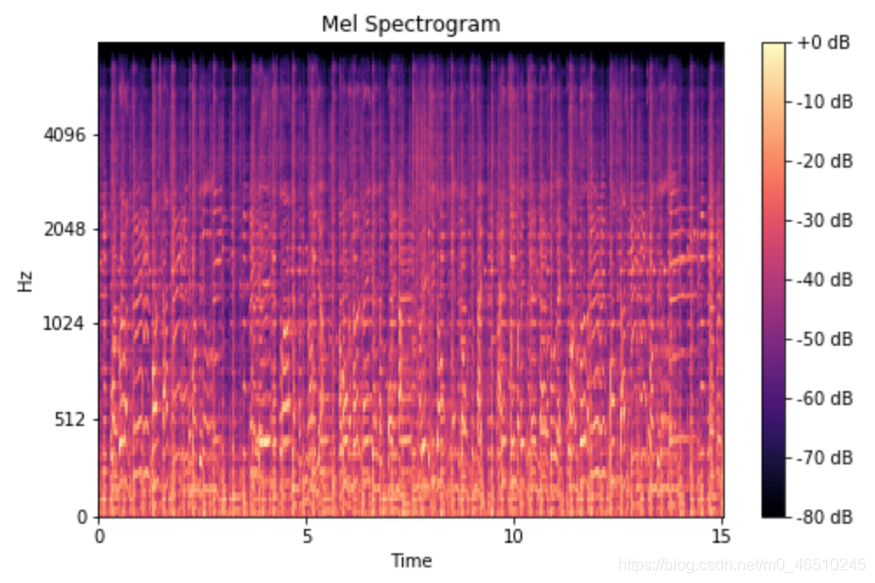
\includegraphics[width=\textwidth]{figures/melPic.png}
      \caption{Mel图}
      \label{fig:Mel}
    \end{figure}
\section{音频数据增强}
\subsection{概述}
音频数据增强最早来自于图像神经网络中的图像增强方法,两者的目的都是为了拓展训练集并鼓励系统对增强过程中的转换保持不变。作为一种补充措施,对系统在转换后的输入上的预测进行学习可以提高针对系统未学习到的样本的鲁棒性。 

在音频数据增强领域,现今的研究成果已经硕果累累了。2013年,Jaitly和Hinton \cite{Jaitly2013VocalTL}率先使用了保留标签的音频转换来进行语音识别。他们发现,在训练和测试时间进行mel滤波之前,频谱图的音调移位会使电话错误率从21.6%降低到20.5%,并报告称按时间或频率维度缩放mel频谱,或者根据扰动的LPC系数构造示例都无济于事。同时,Kanda等人的研究成果\cite{kanda2013elastic}表明,将音调移位与时间拉伸和随机频率失真相结合可将字错误减少10%,而音调移位被证明是最有益的,并且三种失真方法的效果几乎呈线性相加。Xiaodong Cui等人\cite{cui2015data}实现了将音高转换与在特征空间中将语音转换为其他说话者语音的方法结合起来的方法。

在这些研究的基础上,本研究可以确定音频数据增强在提高模型系统性能,避免过度拟合从而提高其通用性。

\subsection{常用的音频数据增强方法介绍及展示}
现今常用的数据增强方法有:加入高斯白噪音、音调转换、时间拉伸、时间平移以及同类音频叠加等。因此本文利用github上的音频数据增强库:audiomentations,展示一些常用的音频数据增强方法,并分析它们的影响。
     \begin{figure}[h]
      \centering
      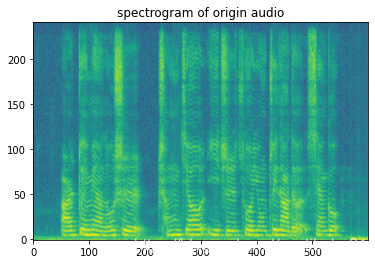
\includegraphics[width=0.5\textwidth]{figures/oasg.png}
      \caption{原始信号的频谱图}
      \label{fig:oasg}
    \end{figure}

按照第一部分介绍的音频特征建模技术,音频数据增强的方法可以用于处理展示频谱图和梅尔频谱图。因为梅尔频谱图需要构建复杂的三角滤波器组,所以本文用频谱图来分析展示数据增强方法,以及这种处理方法的影响。原始信号的频谱图展示如图\ref{fig:oasg}:

分别对原始信号做时间平移、时间拉伸和添加白噪音操作其频谱图变化如图:
    \begin{figure}[h]
      \centering
      \begin{subfigure}{0.3\textwidth}
        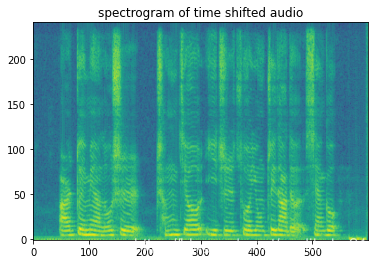
\includegraphics[width=\linewidth]{figures/oats.png}
        \caption{时间平移}
        \label{fig:oats}
      \end{subfigure}
      \begin{subfigure}{0.3\textwidth}
        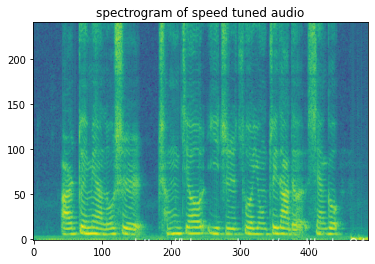
\includegraphics[width=\linewidth]{figures/oast.png}
        \caption{时间拉伸}
        \label{fig:oast}
      \end{subfigure}
        \begin{subfigure}{0.3\textwidth}
        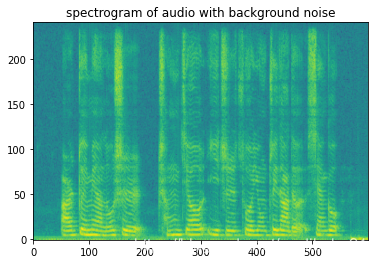
\includegraphics[width=\linewidth]{figures/oabn.png}
        \caption{添加白噪音}
        \label{fig:oabn}
      \end{subfigure}
      \caption{音频数据增强后的频谱图}
      \label{fig:multi-image}
    \end{figure}
    
在audiomentations库中,还有剪切样本、频段屏蔽、质量压缩等音频增强技术的实现。而这些音频增强的方法在最终的模型的影响,将在后面的实验设计过程中进行分析。
\section{迁移学习}
迁移学习是一种微调预训练模型,并快速标记适合的数据的深度学习方法。它与从零开始的深度学习训练相比,微调模型需要更少的标记数据,可以更快的实现训练。
许多迁移学习任务的方法主要有:(i)从一个预先训练的模型开始,(ii)移除特定于任务的顶层,(iii)作为特征提取器对目标任务的底层进行微调。通过这种方法,迁移学习系统可以实现特定任务的特征提取,而本文就采取利用Youtube数据训练的类神经网络VGGish实现基于咳嗽音频的特征提取。
\subsection{研究现状}
Donahue等人在2015年发表的论文\cite{2015The}中确认经过预处理的AlexNet提取的特征可以转移到各种任务中,并且比手工制作的特征工作得更好。Yosinski等人的研究\cite{2014How}表明,微调预训练网络比固定的预训练表征提供更好的性能。即使目标数据集与预先训练的数据集非常不同,微调没有带来性能提高,但可以加快收敛速度。

最近关于迁移学习的研究主要集中在如何更好地利用预训练模型的归纳偏差,即如何利用预训练模型对微调进行规范化。在这些关于迁移学习的研究中都反映了迁移学习作为一种广泛的特征提取方法,有着很好的优势。

\subsection{一般的迁移学习方法}
一般来说,将某一领域的学习模型应用到相关领域是最常见的迁移学习过程。迁移学习方法主要有两种,分别是基于模型的迁移学习以及基于特征的迁移学习。
\begin{enumerate}
    \item \textbf{基于模型的迁移学习}:基于模型的迁移学习主要是基于模型的再学习,经典的模型迁移学习方法就是TrAdaBoost算法,它主要通过增加误分类的目标函数,重新训练数据的权重,同时减少误分类。使得模型更加的适应新方向的数据集。
    \item \textbf{基于特征的迁移学习}:本文主要就是使用基于特征的迁移学习,关注的是哮喘音频领域和人声特征领域的共同特征,然后利用这些特征进行特征映射。
    基于特征映射的迁移学习算法主要研究如何将源域和目标域的数据从原始特征空间映射到新的特征空间。
    这样,在这个空间中,源域的数据分布与目标域的数据分布是一致的,这样就可以更好地利用源域已有的标记数据样本在新的空间中进行分类训练,最终对目标域的数据进行分类测试。
\end{enumerate}
\section{卷积神经网络VGG}
\subsection{概述}
在传统的计算机机器学习中,特征提取往往是最重要的一环。通常机器学习程序员会对原始数据进行各种变形、处理,并人工的选取有代表性的维度。然后利用传统的机器学习分类网络,例如:支持向量机、决策树等进行分类。如果用于分类的特征不具有特异性或者特征点过少,分类器都无法进行有效的分类;而特征点提取过多,又会是分类系统对学习集过拟合,在新样本上的分类能力很差。

由于计算机性能的提高,GPU和大型分布式集群的发展。近年来,卷积神经网络的研究越来越火爆,而利用神经网络系统就仅仅只需要关注网络层的功能和具体的参数限制,而不必太拘泥于数据样本的处理提取,利用网络自动地将自身需要的特征维度提取出来。尤其是ImageNet大规模视觉识别挑战赛(ILSVRC)\cite{russakovsky2015imagenet}已经用作多代大规模图像分类系统的平台,从而导致了深度视觉识别体系结构的许多进步。 

本文将使用Google团队在YouTube数据集上预训练好的VGGish对咳嗽音频进行特征自动提取,因此在本节有必要对卷积神经网络VGG的基本层和算法原理都需要进行简单的分析介绍。
\subsection{VGG的定义和基本层}
Visual Geometry Group(VGG)是一类包含卷积计算并且有深度结构的前馈神经网络(Feedforward Netural Networks)\cite{lecun1998gradient},主要应用于人脸识别、图像分类等方面。下面对卷积神经网络常有的四个基本层及其主要作用。
\begin{enumerate}
\item \textbf{卷积层}:该层主要用于提取输入数据的局部特征。对卷积核(特征提取器)和定义大小的数据执行卷积运算,并且输出层的结果值。一般来说,常用的卷积核有两种:一维卷积核和二维卷积核1。卷积核的大小也决定了局部特征提取的大小。核太小会增加特征维数,核太大会使卷积提取特征的“粒度”不够精细。因此,选择合适的卷积核是非常重要的。
\item \textbf{池化层}:这一层主要是压缩特征维度和减少参数,而不会丢失太多的数据信息。在具体操作中,一般选择合适大小的窗口,并将所有特征值压缩成代表值。一般来说,有两种池方法:最大池和平均池。
\item \textbf{全连接层}:全连接层通常用作卷积层和输出层之间的连接,用于将多维特征值转换为所需的输出值。
\item \textbf{dropout层}:一般添加到全连接层,减少中间特征的数量,防止模型拟合过多,提高模型的泛化能力。
\end{enumerate}

基于以上四种基本层次从高维浅层特征编码到深层ConvNet编码,计算机视觉分类的研究在网络层数上越来越多。但是随着网络深度的增加,会出现更多由降维引发的问题,参数的过多也往往影响着机器学习的效果。
     \begin{figure}[h]
      \centering
      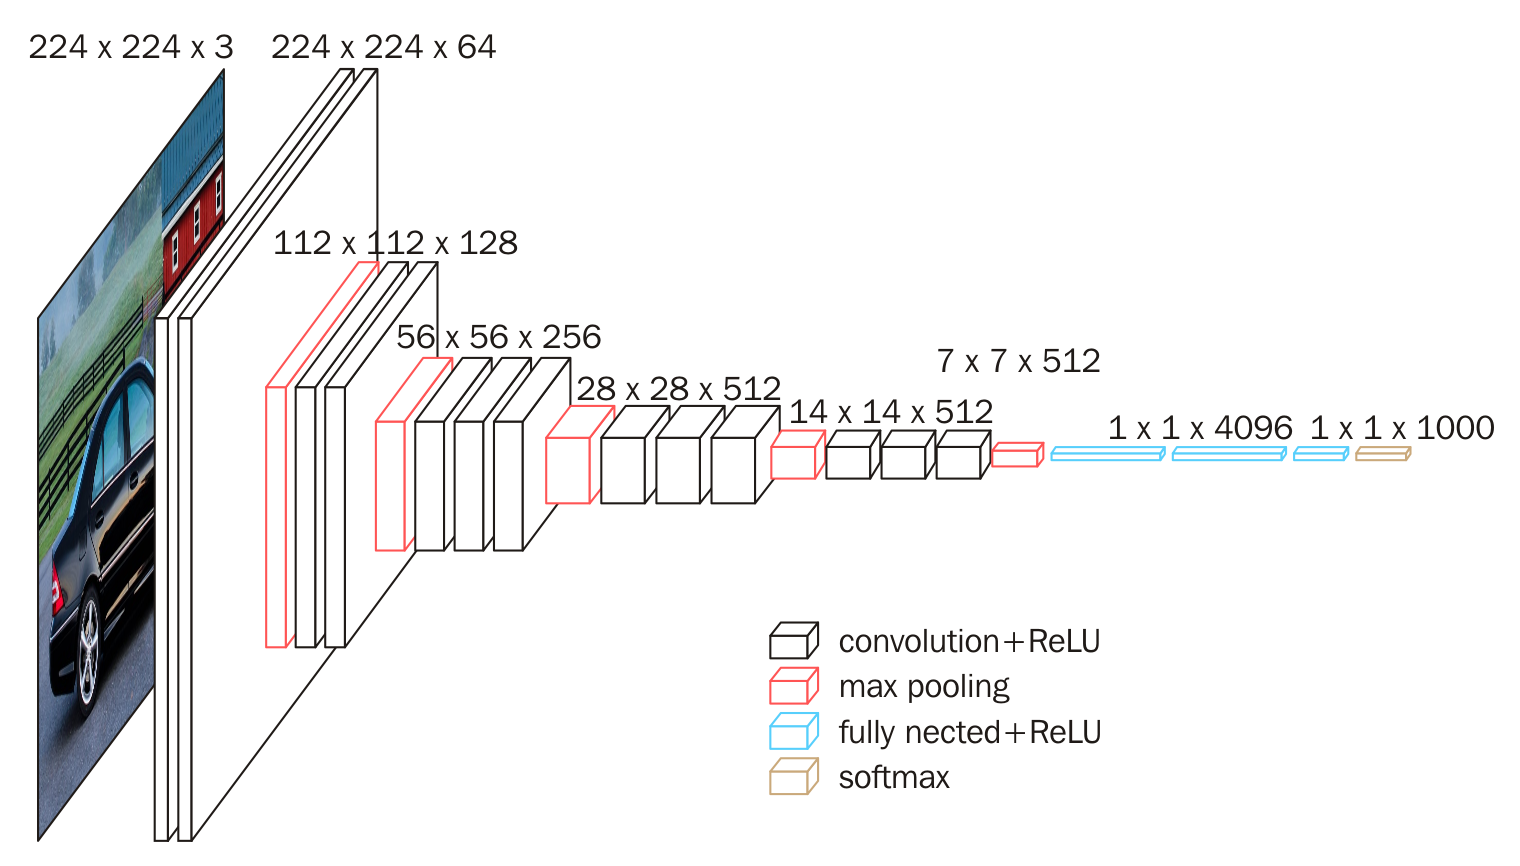
\includegraphics[width=0.7\textwidth]{figures/VGG16.png}
      \caption{VGG16结构示意图}
      \label{fig:vgg16}
    \end{figure}

由此,在2014年ImageNet大规模视觉识别挑战赛上牛津大学基于AlexNet网络提出VGG架构。相对于AlexNet网络,VGG减少了其卷积核的大小。它利用3个\(3\times3\)的卷积核来替代\(7\times7\)的卷积核,使用了2个\(3\times3\)的卷积核替代了\(5\times5\)的卷积核\cite{simonyan2014very}。这种小型的卷积核而不是大型卷积核可以保持更好的图像的性质,VGG16(图\ref{fig:vgg16})就是一种最经典的的VGG网络。

\subsection{VGG16网络结构及特点}
     \begin{figure}[h]
      \centering
      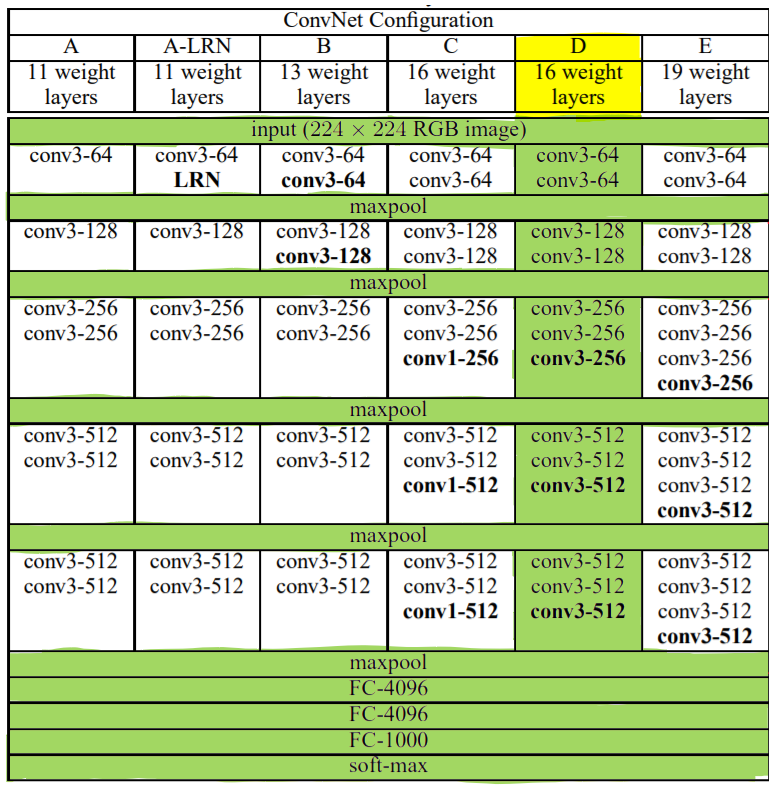
\includegraphics[width=0.6\textwidth]{figures/VGG2.png}
      \caption{VGG常见结构配置}
      \label{fig:vgg2}
    \end{figure}
根据卷积神经网络中卷积核和卷积层数目的不同,如图\ref{fig:vgg2}所示VGG共有六种常见的结构,其中后面两种结构的使用场景最多也最经典。D结构就是本节主要介绍的VGG16


通过对VGG16的结构进行具体分析,其组织结构一共包含以下层:

\begin{itemize}
    \item13层卷积层,在表中以conv3-YYY标号
    \item3层全连接层,在表中以FC-YYY标号
    \item5层池化层,在表中以maxpool标号
\end{itemize}

其中,权重层为卷积层和全连接层,总共有16层,因此此种结构被称为VGG16。

VGG网络的最大特点就是在于简单,因为把所有的大卷积核都缩小为\(3\times3\)的尺寸,并且按照若干层卷积层加上一层池化层的折叠方式,网络结构容易拟合。但是同时VGG16的权重参数有1亿多个,训练和调参难度过大,所以本文直接调用利用YouTube音频数据训练的网络VGGlish提取参数。


% Chapter 3
\chapter{系统设计}

\section{系统总体设计}
本章将介绍基于音频特征建模的哮喘检测系统的实现细节。整个系统的设计架构如图\ref{fig:jiagou}所示:在数据收集阶段,系统收集用户的咳嗽信号后,利用数据增强音频数据,并通过人工音频特征提取和VGGish特征提取。最后将提取到的特征输入SVM分类网络进行分类训练,根据分类指标评估模型的好坏。
\begin{figure}[h]
    \centering
    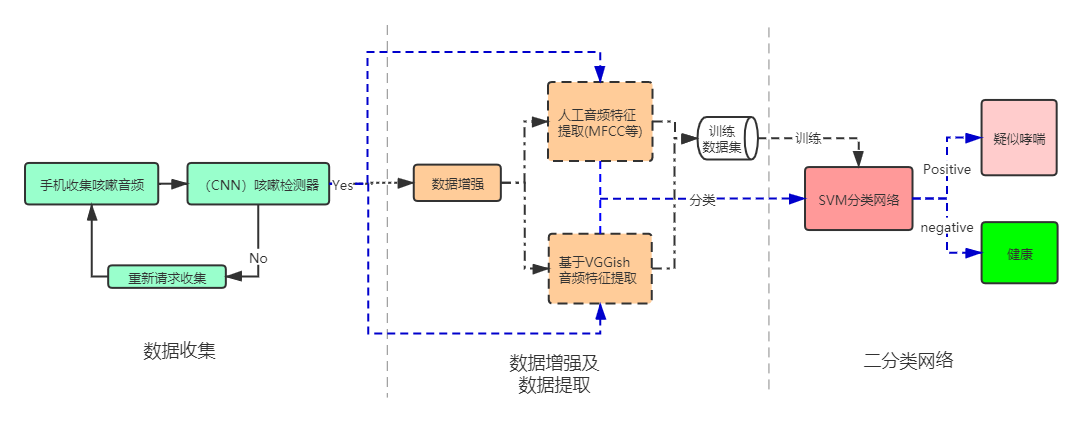
\includegraphics[width=\textwidth]{figures/哮喘检测系统架构.png}
    \caption{哮喘检测系统整体架构}
    \label{fig:jiagou}
\end{figure}

本章主要介绍哮喘检测系统的四个核心部分:(1)利用收集麦克风收集咳嗽音频,并利用CNN神经网络对咳嗽音频的收集结果进行评估;(2)在对咳嗽音频进行音频数据增强后,利用人工处理和VGGish网络进行联合特征提取;(3)SVM分类网络,介绍用于本系统的SVM分类网络架构,简述原因以及分类效果。
\section{原始数据收集及检测}
系统主要基于Android Studio平台搭建了一款收集咳嗽音的手机应用,通过调用手机的麦克风以44.1kHz的采样率对咳嗽音频进行收集,并转化为.wav文件存储到手机本地内存中。但是系统并不能确定原始收集数据是否为咳嗽音频,每一次调用的录音功能都不能保证收集到的数据一定是可用的咳嗽样本。为了使样本满足可用性这一条件,系统需要设计一个简单的CNN网络用于咳嗽样本的检查。

\subsection{咳嗽样本预处理}
根据理论基础中的MFCC理论,系统利用生成咳嗽样本的Mel图用于图像识别分类,处理过程如下:
\begin{enumerate}
    \item 将咳嗽音频重定位至22kHz。
    \item 使用128个Mel成分的三角滤波器对咳嗽音频进行滤波并确定其Mel图。
    \item 调整已经生成的Mel图大小并转化为灰度图,以统一的大小对图像进行缩放并减小图像尺寸,生成\(320\times240\times\)大小的灰度图。
    \item 将生成的图像输入到基于系统的卷积神经网络(CNN)的分类器中,以确定记录的输入声音是否咳嗽
\end{enumerate}

经过系统预处理后的音频图像是一个\(320\times 240 \times 1\)的灰度图,系统用于训练的图展示如图\ref{fig:huidu-image}:其中图\ref{fig:huidu1}为咳嗽音频图像,图\ref{fig:huidu2}和图\ref{fig:huidu3}为其他音源的音频图像。
    \begin{figure}[h]
      \centering
      \begin{subfigure}{0.3\textwidth}
        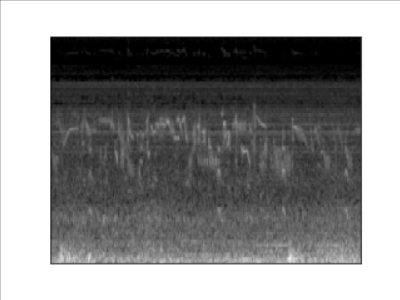
\includegraphics[width=\linewidth]{figures/音频处理1.png}
        \caption{音频灰度图1}
        \label{fig:huidu1}
      \end{subfigure}
      \begin{subfigure}{0.3\textwidth}
        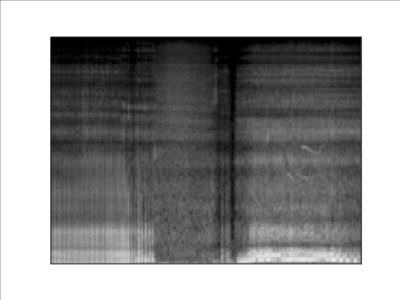
\includegraphics[width=\linewidth]{figures/音频处理2.png}
        \caption{音频灰度图2}
        \label{fig:huidu2}
      \end{subfigure}
        \begin{subfigure}{0.3\textwidth}
        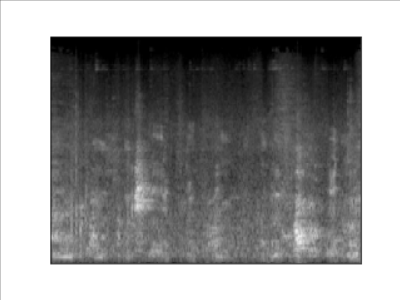
\includegraphics[width=\linewidth]{figures/音频处理3.png}
        \caption{音频灰度图3}
        \label{fig:huidu3}
      \end{subfigure}
      \caption{咳嗽检测训练集样本预处理}
      \label{fig:huidu-image}
    \end{figure}

\subsection{CNN网络结构}
CNN网络的结构设计如图\ref{fig:cnn001},其中包含4个卷积层、3个最大池化层以及1个激活层。最后神经网络生成的2个神经元和softmax激活层用于进行咳嗽与非咳嗽的分类。

\begin{figure}[h]
    \centering
    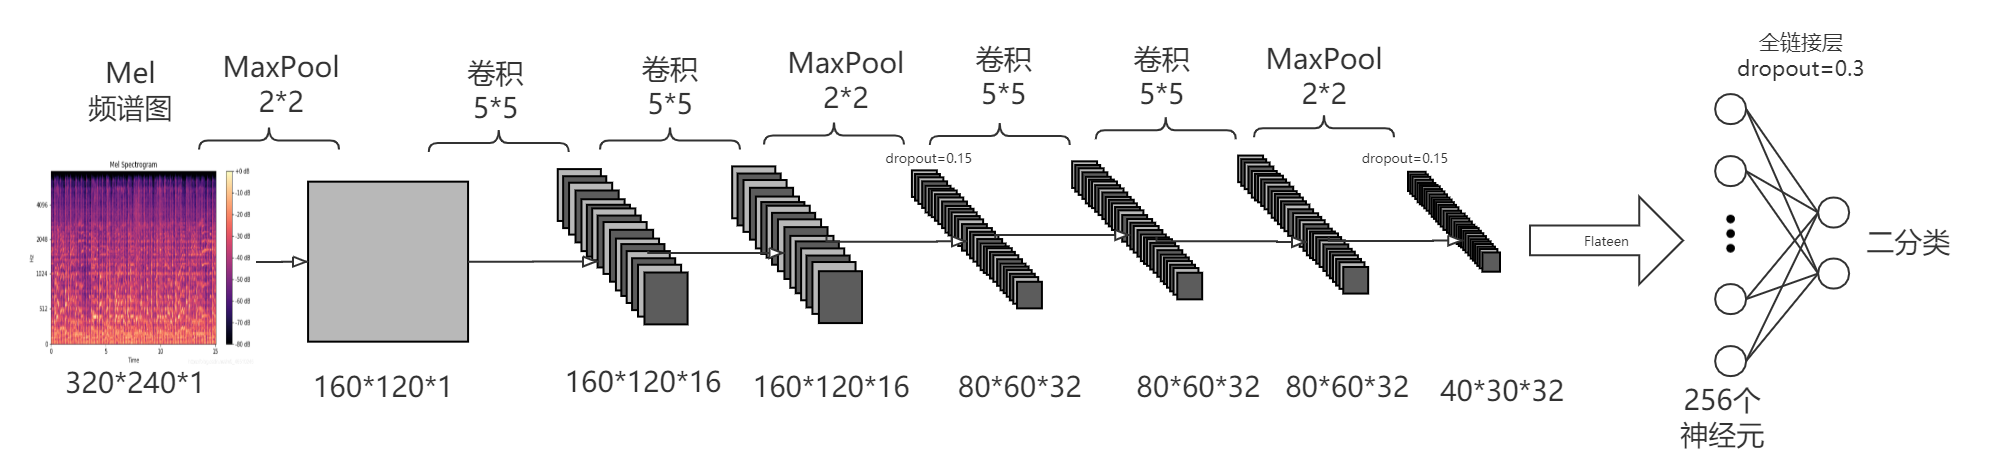
\includegraphics[width=1.1\textwidth]{figures/cnn1.png}
    \caption{咳嗽检测CNN网络}
    \label{fig:cnn001}
\end{figure}

CNN网络的设计思路如下:
\begin{enumerate}
    \item 第一部分是最大池化层。由于输入的Mel光谱图图像尺寸较大,因此在进行下一步之前,首先将其穿过2×2最大池化层以减小整体图像的尺寸,方便进行卷积等特征提取处理。
    \item 第二部分是两个图层块。每个图层包括两个卷积层,并将卷积核大小设置为为5×5,用于提取输入数据的局部特征。其中,第一部分的图层中的卷积层使用了16个过滤器,而第二部分中的两个卷积层使用32个过滤器。系统采用较大的5×5的卷积核是为了减少造成局部特征的过拟合,提高了整体网络的泛化性能与指标。
    \item 第三部分是每个图层块后面的一个2×2的最大池化层以及一个系数为0.15的Dropout层。最大池化层是为了进一步减小图像尺寸,而Dropout层是为了随机让网络某些隐含层节点的权重不对合并进行产生影响,提高整体神经网络的可靠性。
    \item 第四部分是一个完全连接层。系统将从这4个卷积层中学习到的复杂特征进行展平处理,传递到具有256个神经元的完全连接层,最后利用系数为0.3的Dropout层继续防止过拟合情况的发生。
    \item 最后一部分是2个神经源和softmax激活功能的输出层。通过这层结构系统就可以完成对给定输入的咳嗽与非咳嗽音频进行分类。
\end{enumerate}

同时对于该神经网络系统还有一些实现的细节。在该模型中,系统使用ReLU函数作为所有卷积层的激活函数,并利用Adam优化器优化神经的网络结构\cite{kingman2015adam}以及使用交叉熵损失函数作为卷积网络的损失函数。

\section{特征提取}
由于本文使用的数据量较小,系统将采用基于特征的机器学习来提取音频信号的特征向量。系统实现了传统的手工设计特征和迁移学习两种不同的特征提取方法,并使用主成分分析法对系统所有提取到的特征进行降维处理。

\subsection{手工设计特征}
对于咳嗽音频
接下来系统将指明本文挑选的特征值以及挑选的原因
\begin{enumerate}
    \item \textbf{短时平均过零率(Zero Crossing Rate)}:ZCR是指一定时间内音频波形通过直线y=0的次数。这个给特征值在一定程度上反映了频率的大小。ZCR低的音频一般比较浑浊,而ZCR高的音频则比较清澈,因此短时平均过零率用于初步分析清晰、浑浊的音频。通过因为短时平均过零率容易受到低频噪音的干扰,为了提高鲁棒性,系统会在处理中添加阈值,即波形穿过阈值的次数被定义为短时平均过零率。计算算法如下:
\begin{algorithm}[h]
    \caption{ ZCR计算} %算法的名字
    \hspace*{0.02in} {\bf Require:}\\%算法的输入, 
    采样率:fs,一段时间的音频信号:f(t),帧长:wlen,帧移:inc,阈值:\(\alpha\)\\
    \hspace*{0.02in} {\bf Ensure:} %算法的结果输出
    \begin{algorithmic}[1]
    \State 消除直流分量  f(t) = f(t)-mean(f(t)) % \State 后写一般语句
    \State 初始化 wlen = 200, inc = 80, count=0, \(\alpha\)=0.05*max(f(t))
    \State 分帧F, 获取帧数fn
    \State \textbf{for} i = 1:fn \textbf{then}
      \State z=F[i]
      \State \textbf{for} i = 1:(wlen-1) \textbf{then}\\
                \textbf{if} z(j)*z(j+1)<\(\alpha\) \textbf{then}\\
                    count++;\\
        \textbf{end}\\
        \textbf{end}\\
    \textbf{end}
    \State \Return count
    \end{algorithmic}
\end{algorithm}
    \item \textbf{短时音频能量}:短时音频能量是音频信号相应的帧长归一化的振幅值的平方和,依然是用来分辨清澈和浑浊音频的的指标,在时刻T,其计算公式如下:
    \begin{equation}
        E_n = \sum_{m=t-(N-1)}^{t} F[m]^2
    \end{equation}
    \item \textbf{能量熵}:系统将子帧归一化后取其能量的熵,用来度量音频中突变音的发生。
    \item \textbf{共振峰频率}:共振峰是由人声道的共振引起的频谱整形。
    \item
    \textbf{峰度}:峰度是对实值随机变量的概率分布的右部分的度量。
    \item
    \textbf{RMS能量}:RMS能量是信号功率的短时傅里叶变换幅度的均方根,用于表征信号中的能量大小。
    \item
    \textbf{频谱质心}:功率谱图每帧功率的平均值(即质心)。
    \item
    \textbf{截止频率}:功率谱图的中心频率,以便此帧中至少85\%的频谱能量包含在该值及以下。
    \item
    \textbf{MFCC}:MFCC反映了频谱的轮廓,系统基于非线性Mel尺度上对数功率谱的线性余弦变换,从短期功率谱获得Mel频率倒谱系数。系统使用前13个分量的值。
    \item
    \textbf{\(\Delta\)-MFCC}:MFCC的时间微分
    \item
    \textbf{\(\Delta^2\)-MFCC}:MFCC增量的微分(加速度系数)
\end{enumerate}

对于产生的具有时间性质的特征(如:均方根能量、频谱质心、截至频率和MFCC的所有变体),系统提取了一些统计特征,以便捕捉超出平均值的分布。包括:平均值,中位数,均方根,最大值,最小值,1/4位数和3/4位数,四分位的间距,标准差,偏度,峰度。总共有477个手工设计特性,包括3个段级特性、4个由其统计数据表示的帧级特性和3个MFCC的特征,每个组件由其统计数据表示(3+4)× 11 + 3 × 13× 11 = 516。
\subsection{迁移学习特征}
除了手工设计的特征外,系统还使用VGGish来自动提取音频特征[15]。
VGGish是一个卷积神经网络,主要用于基于原始音频输入的音频分类。VGGish是使用大型YouTube数据集进行了训练的模型,并公开发布了学习到的模型参数。因此本系统将其用作特征提取器,将原始音频波形转换为嵌入(特征),然后将其传递以训练SVM分类器。具体训练方法如下:
\begin{enumerate}
    \item 将音频重采样为 16kHz 单声道,
    \item 使用 25ms 的帧长、10ms 的帧移,以及 Hann 窗口对咳嗽音频进行分帧,切割为0.96s的非重叠子帧
    \item 对每一帧做傅里叶变换,然后利用信号幅值计算声谱图
    \item 通过将声谱映射到 64 阶 mel 滤波器组中计算 mel 声谱,并对声谱图取对数能量
    \item 模型每0.96秒返回128维特征向量,将整个线段的均值和标准差作为最终特征,尺寸为256(128×2)
\end{enumerate}

需要注意的是由于VGGish仅基于频谱图输入,因此时域中的一些重要特征可能会在特征空间中遗漏。

\section{支持向量机}
\subsection{概述}
支持向量机(support vectormachines)是机器学习中最经典的二分类模型。这种分类器提供了一种有监督的学习模型,该模型在训练后得到一个最大分离两类的超平面决策边界。

一般来说,为了处理非线性可分的数据,SVM可以加入适当的核,将原始特征空间转换为高维空间,在高维空间中,转换后的特征成为线性可分的(见图4的解释说明)。形式上,选择决策超平面\(w^Tφ(x) + b = 0\)(其中φ(x)表示变换特征空间中的一个点向量,φ为核函数,w为权向量,b为偏差)来最大化整体分离。相当于最大化公式\ref{eq:svm}
\begin{equation}
    \label{eq:svm}
    \sum_{i=1}^n \alpha_i -0.5\sum_{i=1}^n \alpha_i \alpha_j y_i y_j K(x_i,x_j)
\end{equation}

其中\(a_i \ge 0,i=1,2,...n\),且\(\sum_{i=1}^n\alpha_i y_i=0\)。对于每一个数据的索引i,\(x_i,y_i\)分别表示特征向量和对应类的标签(+1代表正样本,-1代表负样本),并且K表示核函数,n表示数据集的大小,\(\alpha_i\)代表拉格朗日乘数。

本理论介绍两类支持向量机的分类性能,其中一种向量机的核函数为线性核(即:\(K(x_i, x_j) = x_i^T x_j\)),另一种的核函数是径向基函数(即\(K(x_i,x_j) = exp \frac{|x_i-x_j|^2}{2σ^2})\),这是一种泛在非线性核。

\subsection{性能表现}
为了评估分类性能,SVM参数,即权重向量w和偏差b,在数据子集(训练子集)上进行优化,并针对互补(测试)子集进行验证。准确地说,数据集被划分为训练和测试的子集,这样:(1)他们大小的比率,称为训练-测试比率,这是一个预先分配好的参数;(2)这些子集中健康以及患病的比例也大致于训练-测试比率相同。一般情况下,分类器的性能取决于主观选择的分割条件。为了避免性能分析中这种主观性,通常使用蒙特卡罗交叉验证(MCCV)\cite{2001Monte},如图\ref{fig:MCCV}所示,本文的所有数据集被随机划分大量(5000)次(迭代),并分割比和前面提到的训练-测试比例保持不变。在每一次迭代,SVM参数在训练子集上进行优化,并记录平均训练、测试精度和相应的标准差。
\begin{figure}
    \centering
    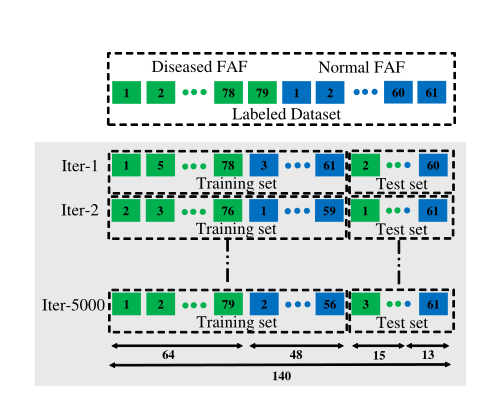
\includegraphics{figures/MCCV.PNG}
    \caption{MCCV方法流程}
    \label{fig:MCCV}
\end{figure}

值得注意的是,训练精度表明了当前模型对可见数据的分类性能,而测试精度表明,对于不可见数据,平均测试精度高的分类器具有实际意义。此外,低标准差(该情况表明在随机分区上的低可变性,从而表明系统的健壮性)是可取的。并且通过计算了超过5000次迭代的平均混淆矩阵,系统提供了健康类和疾病类的每个类条件检测概率。最终实验环节实验组训练和观察了SVM分类器不同的训练-测试比率对SVM性能的影响。
% Chapter 4
\chapter{实验设计及其结果}
\section{实验准备}
为了成功完成哮喘检测实验,系统需要准备的工具有:Android应用程序(用来收集咳嗽音频,并存储在本地内存中)以及装有tensorflow和matlab环境的笔记本电脑(用来提取音频特征并进行对音频进行分类)

在实验数据采集阶段,本人联系了武汉市中南医院呼吸科找到了4名患有哮喘的病人分别采集了10min左右的咳嗽信号,并利用咳嗽检测网络筛选了300组有效的单周期咳嗽信号,作为本系统的正样本数据。紧接着本人联系了5名身体健康的志愿者共收集了500组负咳嗽样本数据。
\section{咳嗽检测网络测试}
对应已经收集到的咳嗽信号,系统要对咳嗽事件进行正确的检测,去除样本中噪音大或者非咳嗽的样本,因此系统需要训练一个鲁棒性良好的咳嗽检测网络。

本网络的数据是使用Kvapilova L等人\cite{kvapilova2019continuous}的采集咳嗽样本作为正样本进行训练,将咳嗽样本与一些背景噪声混合以使其更加真实,从而达到扩大数据集的目的,背景噪音来自于musan数据集\cite{musan2015},其中噪音比为0.15。最终系统利用在数据采集阶段收集到的咳嗽样本(包括正常人咳嗽样本和病人咳嗽样本)对真实的样本进行分类检测。来观察训练出的网络对真实样本分类的有效性。
\subsection{参数重要性分析}
系统利用初步网络训练对参数的重要性和相关度进行分类。
\begin{table}[h]
\centering
\begin{tabular}[width=0.6\textwidth]{ccc}
\hline
\textbf{参数}                           & \textbf{重要性}                                     & \textbf{相关度}                                      \\ \hline
{\color[HTML]{343434} \textbf{drop1}} & {\color[HTML]{6434FC} \textbf{0.041}}            & {\color[HTML]{009901} \textbf{0.243}}             \\
\textbf{conv3}                        & {\color[HTML]{6434FC} \textbf{0.063}}            & {\color[HTML]{009901} \textbf{0.133}}             \\
conv2                                 & {\color[HTML]{6434FC} 0.071}                     & {\color[HTML]{009901} 0.124}                      \\
\textbf{drop2}                        & {\color[HTML]{6434FC} \textbf{0.038}}            & {\color[HTML]{009901} \textbf{0.091}}             \\
\textbf{conv4}                        & {\color[HTML]{6434FC} \textbf{0.047}}            & {\color[HTML]{009901} \textbf{0.089}}             \\
batch\_size                           & {\color[HTML]{6434FC} 0.041}                     & {\color[HTML]{009901} 0.041}                      \\
lr                                    & \multicolumn{1}{l}{{\color[HTML]{6434FC} 0.048}} & \multicolumn{1}{l}{{\color[HTML]{009901} 0.028}}  \\
conv1                                 & \multicolumn{1}{l}{{\color[HTML]{6434FC} 0.050}} & \multicolumn{1}{l}{{\color[HTML]{FE0000} -0.021}} \\
pool1                                 & \multicolumn{1}{l}{{\color[HTML]{6434FC} 0.432}} & \multicolumn{1}{l}{{\color[HTML]{FE0000} -0.113}} \\
beta2                                 & \multicolumn{1}{l}{{\color[HTML]{6434FC} 0.013}} & \multicolumn{1}{l}{{\color[HTML]{FE0000} -0.121}} \\
alpha                                 & \multicolumn{1}{l}{{\color[HTML]{6434FC} 0.050}} & \multicolumn{1}{l}{{\color[HTML]{FE0000} -0.257}} \\
beta1                                 & \multicolumn{1}{l}{{\color[HTML]{6434FC} 0.106}} & \multicolumn{1}{l}{{\color[HTML]{FE0000} -0.274}} \\ \hline
\end{tabular}
\caption{模型参数重要性分析}
\end{table}

该表显示了不同的超参数对“真实样本准确率”的影响。第一列显示了参数的重要性,第二列显示了与参数更改量之间的相关性,以及参数增加是否改善或恶化了参数。通过准确性得分,系统可以看到\(\beta_1\)、\(\beta_2\)以及\(\alpha\)对系统的影响很小,因为没有任何变化带来了性能提升。但同时几个卷积层以及损失函数对本网络的数据影响很大,但尚未经过足够的测试,应对此进行调查。
\subsection{模型参数调整}
本节为对于咳嗽检测网络进行网络模型训练的参数调整确认。通过调整系统的参数,实验验证了不同的系统参数对于模型的影响。

由上节的分析系统可以看出参数中卷积层的大小以及损失函数对模型的效果影响最大。所以需要选取适宜的网络的损失函数和子图数目。通过初步筛选,系统将损失函数确定为:交叉熵损失函数和最大似然损失函数两种。假定训练时所有条件均保持不变,按照第三章的网络结构进行设计,即在卷积核大小为\(5\times5\),池化核大小为\(2\times2\),训练集为1800,batch数目为128,训练次数为50,优化器采用Adam的条件下进行训练对比,其结果如下:
\begin{table}[h]
\centering
\begin{tabular}{cccc}
\hline
\textbf{损失函数/子图数}                                 & \textbf{验证集准确率}                        & \textbf{训练集准确率}                        & \textbf{真实样本准确率}                       \\ \hline
{\color[HTML]{FE0000} \textbf{交叉熵/(16,16,32,32)}} & {\color[HTML]{FE0000} \textbf{0.9756}} & {\color[HTML]{FE0000} \textbf{0.9673}} & {\color[HTML]{FE0000} \textbf{0.8941}} \\
交叉熵/16,16,16,32                                   & 0.9732                                 & 0.9682                                 & 0.8888                                 \\
最大似然/16,16,32,32                                  & 0.9672                                 & 0.969                                  & 0.8574                                 \\
交叉熵/32,32,32,32                                   & 0.9731                                 & 0.9663                                 & 0.862                                  \\
最大似然/16,16,16,32                                  & 0.9142                                 & 0.9008                                 & 0.708                                  \\
最大似然/32,32,32,32                                  & 0.9678                                 & 0.9669                                 & 0.8914                                 \\ \hline
\end{tabular}
\caption{调整损失函数和子图数对模型的影响}
\end{table}

通过表格系统可以看到当系统使用交叉熵函数作为系统的损失函数且子图数选取为16,16,32,32时样本分类准确性和真实数据分类准确率最高,到达了89.4\%基本适用于进行咳嗽的检测。
\subsection{模型决策修正}
在模型参数调整阶段,系统已经将真实样本的决策准确率提高到89\%。系统可以知道单周期的咳嗽音频信号可能难以特别准确分类(到达99\%)以上,所以说系统修改分类判断,对一段时间内多次的连续的咳嗽信号进行联合分类判断,用于修正模型的决策过程,具体理论以及决策过程如下:
\begin{enumerate}
    \item 存储连续N个连续的咳嗽音频信号,进行单周期的分类决策。
    \item 如果N个信号中,有T个信号及其以上的信号判断一致时,系统采取该判定值为本次连续分类决策的最终结果。
    \item 否则回到第一步,重新存储N个连续信号,进行联合分类决策
\end{enumerate}

在上述的理论情况下,系统使用公式\ref{eq:3.3}估算当N=3,T=2时联合分类决策的错误率:
\begin{equation}
    \label{eq:3.3}
    ErrorRate = C_4^3\times(0.11)^3\times0.89+0.11^4 \approx 0.488477\%
\end{equation}
以上理论表明,即使单周期咳嗽音信号的识别率在89\%左右,但是通过四次连续的联合分类决策,可以将识别率提升到99.5\%左右,系统按照此方法对网络进行训练以及预测,其网络结果如\ref{fig:xunlian-image}。最终的分类成功率在99\%左右。
    \begin{figure}[h]
      \centering
      \begin{subfigure}{0.4\textwidth}
        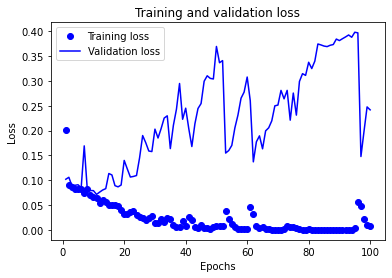
\includegraphics[width=\linewidth]{figures/100.png}
        \caption{训练阶段损失函数变化}
      \end{subfigure}
      \begin{subfigure}{0.4\textwidth}
        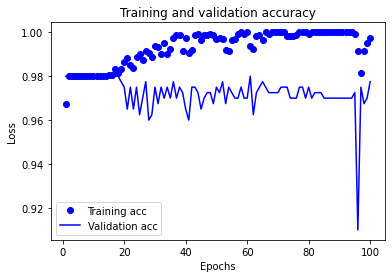
\includegraphics[width=\linewidth]{figures/100轮 准确性.png}
        \caption{训练阶段准确率变化}
      \end{subfigure}
      \caption{CNN训练过程展示}
      \label{fig:xunlian-image}
    \end{figure}
\section{支持向量机网络测试}

特征提取系统结构中论述所示,系统通过人工设计特征以及迁移学习获取了700多维度的特征向量并使用PCA降维最终形成长度为118的特征向量。如前所述,系统考虑了两种不同的支持向量机分类器,线性支持向量机和带RBF核的支持向量机(RBF-SVM)进行性能比较。在每一种情况下,训练和测试的准确性值被记录在大量(5000)的随机分区中,对于在10:90和90:10之间选择的各种训练测试的划分比,其平均值(标准差在括号中)列于表中。

\begin{table}[h]
\caption{样本相同,不同训练测试集划分比,不同SVM的分类结果}
\begin{tabular}{c|cc|cc}
\hline
                                     & \multicolumn{2}{c|}{\textbf{线性SVM}}                         & \multicolumn{2}{c}{\textbf{RBF-SVM}}                                          \\ \cline{2-5} 
\multirow{-2}{*}{\textbf{训练-测试集合比率}} & \textbf{训练集准确率}              & \textbf{测试集准确率}              & \textbf{训练集准确率}                       & \textbf{测试集准确率}                       \\ \hline
{\color[HTML]{343434} 10:90}         & {\color[HTML]{333333} 91.27} & {\color[HTML]{333333} 75.03} & {\color[HTML]{333333} 99.38}          & {\color[HTML]{333333} 78.97}          \\
20:80                                & {\color[HTML]{333333} 91.51} & {\color[HTML]{333333} 82.26} & {\color[HTML]{333333} 98.81}          & {\color[HTML]{333333} 84.32}          \\
30:70                                & {\color[HTML]{333333} 92.04} & {\color[HTML]{333333} 85.56} & {\color[HTML]{333333} 97.88}          & {\color[HTML]{333333} 86.66}          \\
40:60                                & {\color[HTML]{333333} 92.26} & {\color[HTML]{333333} 87.31} & {\color[HTML]{333333} 98.86}          & {\color[HTML]{333333} 88.11}          \\
50:50                                & {\color[HTML]{333333} 92.24} & {\color[HTML]{333333} 88.40} & {\color[HTML]{333333} 98.86}          & {\color[HTML]{333333} 88.89}          \\
60:40                                & {\color[HTML]{333333} 92.27} & {\color[HTML]{333333} 89.02} & {\color[HTML]{333333} 98.46}          & {\color[HTML]{333333} 89.58}          \\
70:30                                & {\color[HTML]{333333} 92.31} & {\color[HTML]{333333} 89.53} & {\color[HTML]{333333} 98.62}          & {\color[HTML]{333333} 90.10}          \\
80:20                                & {\color[HTML]{333333} 92.26} & {\color[HTML]{333333} 89.88} & {\color[HTML]{333333} 98.65}          & {\color[HTML]{333333} 90.55}          \\
90:10                                & {\color[HTML]{333333} 92.25} & {\color[HTML]{333333} 89.60} & {\color[HTML]{333333} \textbf{98.86}} & {\color[HTML]{333333} \textbf{90.83}} \\ \hline
\end{tabular}
\end{table}

显然,对于线性支持向量机,平均训练和测试准确率水平随着训练测试比的增加而增加,但也有少数例外。正如预期,随着训练数据的可用性的增加,该分类器往往学习得更好。对于RBF-SVM模型中,系统所得到的平均测试精度,仍然很大程度上遵循上述增加的趋势,比使用线性支持向量机获得的每个分裂比略有改善。这表明了潜在问题中固有的中等程度的非线性。尽管在测试精度上只有轻微的提高,但平均训练精度的提高明显更高,这表明RBF核在建模方面训练数据的某些非线性方面,而这些方面不能很好地一般化划分。

实际上,考虑标准差值也可以得出类似的结论如下。在线性SVM和BBF-SVM两种模型中训练精度的标准差都随着划分比的增加而减小,并且后者的值明显更低,表明RBF-SVM建模效果更好。然而,从测试精度来看,当划分比值较低时,RBF-SVM的标准差较低,当划分比值较高时,线性SVM的标准差较低。这一现象表明系统泛化性能较差。随着划分比的增加,两种情况下的标准差先减小后增大可以看出细微的差别。而测试的准确性是最可靠的(即,具有最低的标准偏差),在线性SVM的情况下(也在[26]其他地方观察到)一个均匀的划分训练测试比,在RBF-SVM的情况下,最高的可靠性是在划分比40:60观察到。
\begin{table}[h]
\centering

\begin{tabular}{cccc}
\hline
\multicolumn{1}{l}{{\color[HTML]{000000} }}      & {\color[HTML]{000000} \textbf{预测\textbackslash{}真实}} & {\color[HTML]{000000} \textbf{哮喘}} & {\color[HTML]{000000} \textbf{健康}} \\ \hline
{\color[HTML]{000000} }                          & {\color[HTML]{000000} 哮喘}                            & {\color[HTML]{000000} 89.47}       & {\color[HTML]{000000} 7.75}        \\
\multirow{-2}{*}{{\color[HTML]{000000} 线性SVM}}   & {\color[HTML]{000000} 健康}                            & {\color[HTML]{000000} 10.53}       & {\color[HTML]{000000} 92.25}       \\
{\color[HTML]{000000} }                          & {\color[HTML]{000000} 哮喘}                            & {\color[HTML]{000000} 91.61}       & {\color[HTML]{000000} 11.41}       \\
\multirow{-2}{*}{{\color[HTML]{000000} RBF-SVM}} & {\color[HTML]{000000} 健康}                            & {\color[HTML]{000000} 8.39}        & {\color[HTML]{000000} 88.59}       \\ \hline
\end{tabular}
\caption{训练测试集划分比为80:20的预测混淆矩阵(\%)}
\end{table}

虽然对于健康类,线性支持向量机在准确性和可靠性方面略优于RBF-SVM。请注意,给定疾病类别的RBF-SVM相对于线性SVM的优势与给定健康类别的线性SVM相对于RBF-SVM的优势是相似的。然而,由于给出患病类比给出健康类会产生更高的实际代价,因此应该选择RBF-SVM作为筛选工具。

综上考虑系统用80:20划分条件下,RBF-SVM的支持向量机。此时RBF-SVM对健康类的正确率为\textbf{88.59\%}对于哮喘类的正确率为\textbf{91.61\%},标准差分别为\textbf{7.09\%}和\textbf{8.82\%}。
% chapter 5
\chapter{总结与展望}
\section{论文工作总结}
在本文中系统研究了基于咳嗽音频的哮喘检测方式,由于系统的检测方式是基于Android平台搭建的,而不需要专业的检测机器,因此对比其他很多的哮喘诊断方法具有更好的实用性和普查性。系统再此研究的背景下研究了音频中咳嗽事件的检测、迁移学习实现特征提取以及支持向量机份分类的性能问题。

对于音频中咳嗽事件的检测问题,系统提出建立一个CNN网络进行咳嗽事件的检测。该网络是利用Kvapilova等人数据库的采集咳嗽样本加以环境噪音进行训练的。系统通过分析网络参数的重要性和相关性后,将网络性能的重点聚焦于特征子图的个数以及损失函数的选取。最终通过分析确定了损失函数为交叉熵损失函数,特征子图个数为16,16,32,32,并经过联合分类决策,极大地提高了检测网络的可靠性。

对于迁移学习问题,系统使用Youtube数据集训练的类神经网络VGGish提取咳嗽音频数据的特征向量,但是因为VGGish仅基于频谱图输入进行特征提取,会遗漏时域中的一些重要特征,因此系统还采用了人工设计的方式提取了新的500维特征向量,保证了特征空间的全面性和准确性

最后对于支持向量机的分类性能问题,系统主要分析了线性支持向量机和带RBF核的支持向量机(RBF-SVM)的性能比较关系。由于系统提取到的特征向量维度较高且重点不突出,系统采取PCA方法对特征向量进行降维处理,并分析不同训练比对两类向量机性能的影响,最终系统选取了训练集-测试集80:20的情况并采用RBF-SVM进行特征分类,达到了90\%以上的分类效率。

综上所述本研究主要实现一种基于咳嗽音频的哮喘检测方式,通过手机麦克风收集用户的咳嗽音频,并在经过音频数据增强后,利用联合特征提取和VGG模型特征提取,提取一个733维度的特征向量,将所有的特征点进行主成分分析法(PCA)降维处理后,使RBF支持向量机进行二分分类,分类准确率平均达到90\%以上。

\section{下一步工作}
虽然本论文的最终分类准确率达到了90\%以上,但是本研究的局限性也很大。首先是音频提取的负样本不够全面,没有办法很好的涵盖各种环境下咳嗽音的检测,在环境噪音较大的情况下决策失败率很高,需要多次采样。未来改进的方法主要有以下两种:1.使用VGGish模型对咳嗽事件检测采取小样本学习;2.继续加大负样本量,通过数据增强等方式,提高模型的鲁棒性

其次在哮喘检测的工作中,只是简单的对哮喘健康进行分类,而没有对其他异常咳嗽情况进行检测和分类。在测试样本中,有一名志愿者没有患有哮喘但是近期有咽炎症状,分类效果并不良好,因此在上面的分类实验中,已经去除该志愿者的实验数据。为了提高系统的冗余性,该研究的下一步工作就是去寻找其他几种常见异常咳嗽病人进行细分类。

\end{document}